\chapter{Cascade of regulation - The Langevin equation}
\label{ch:langevin}

\section{Intrinsic noise in a single gene using the Langevin approach}
\label{sec:lan-single}
In the Langevin approach, a term representing the noise of the system is added to the deterministic equations instead of considering the transition rates between states explicitely. Knowing some of the statistical properties of the noise term will allow us to find the noise in the number of species. In this section we use the Langevin approach to find the noise for a single gene.

Consider the model used on section \ref{sec:mas-single_gene}. For each of the deterministic equations [eqs. \eqref{eq:mas-simple_det_1}] a stochastic process $\mu(t)$ is added that accounts for the noise. Including the terms $\mu_1(t)$ and $\mu_2(t)$ results in

\begin{equation}
  \label{eq:lan-simple_1}
  \begin{split}
    \dot{n_1}(t) &= k_rd-\gamma_rn_1(t) + \mu_1(t),\\
    \dot{n_2}(t) &= k_pn_1(t)-\gamma_pn_2(t) + \mu_2(t).
  \end{split}
\end{equation}

Now $n_1(t)$ and $n_2(t)$ are stochastic processes. We need some information about the noise terms in order to proceed. First, as we saw in chapter \ref{ch:master}, the averages must follow the deterministic behavior. By taking averages on both sides of eqs. \eqref{eq:lan-simple_1} and imposing this condition we get

\begin{equation*}
  \langle\mu_1\rangle(t) = \langle\mu_2\rangle(t) = 0.
\end{equation*}

Also, assuming white noise statistics, the autocorrelations are given by

\begin{align}
  \langle\mu_1(t)\mu_1(t+\tau)\rangle &= q_1^2\delta(\tau),\label{eq:lan-simple_cor1} \\
  \langle\mu_2(t)\mu_2(t+\tau)\rangle &= q_2^2\delta(\tau). \label{eq:lan-simple_cor2}
\end{align}

Hence, we are assuming that there is no correlation between the values of the noise term at different times. The coefficients $q_1$ and $q_2$ determine the strenght of the noise and will be treated later. Also, the intrinsic noise must be fully uncorrelated among mRNA and proteins, thus

\begin{equation}
  \langle\mu_1(t)\mu_2(t+\tau)\rangle = 0. \label{eq:lan-simple_cor12}
\end{equation}

We use eqs. \eqref{eq:lan-simple_cor1} - \eqref{eq:lan-simple_cor12} to find the noise in mRNA and protein numbers. Define the difference with respect to steady state average as $\delta n_1$ and $\delta n_2$, i.e. $\delta n_i \coloneqq n_i - \langle n_i\rangle_s$, for $i=1,2$. In terms of these quantities eqs. \eqref{eq:lan-simple_1} become

\begin{align*}
  %\label{eq:lan-simple_d1} \label{eq:lan-simple_d2}
  \dot{\delta n_1}(t) &= -\gamma_r\delta n_1(t) + \mu_1(t),\\
  \dot{\delta n_2}(t) &= k_p\delta n_1(t) -\gamma_p\delta n_2(t) + \mu_2(t).
\end{align*}

Fourier transforming and using the fact that $\left[\mathscr{F}(\dot{x}(t))\right](\omega) = i\omega \hat{x}$, where $\hat{x}\coloneqq\mathscr{F}(x)$ we get 

\begin{equation}
  \label{eq:lan-nfourier}
  \delta\hat{n}_1(\omega) = \frac{\hat{\mu}_1(\omega)}{\gamma_r+i\omega},\quad\quad \delta\hat{n}_2(\omega) = \frac{\delta\hat{n}_1(\omega) + \hat{\mu}_2(\omega)}{\gamma_p+i\omega}.
\end{equation}

Taking the average of the square norm of the first expression we obtain the power spectrum for $\delta n_1$

\begin{equation}
  \label{eq:lan-simple_psd1}
  \langle|\delta\hat{n}_1|^2\rangle = \frac{\langle|\hat{\mu}_1|^2\rangle}{\omega^2+\gamma_r^2} = \frac{q_1^2}{\omega^2+\gamma_r^2},
\end{equation}

because from the Wiener-Khinchin theorem [eq. \eqref{eq:con-wkth}] and eq. \eqref{eq:lan-simple_cor1} we obtain $\langle|\hat{\mu}_1|^2\rangle = q_1^2$. Applying the inverse Fourier transform and evaluating at $t=0$ yields the variance of $n_1$ in steady state

\begin{equation}
  \label{eq:lan-qrel1}
  \sigma^2(n_1) = \langle\delta n_1^2\rangle = q_1^2 \left[\mathscr{F}^{-1}\left(\frac{1}{\omega^2+\gamma_r^2}\right)\right](t=0) = q_1^2\int_{-\infty}^\infty\frac{1}{\omega^2+\gamma_r^2}\frac{\mathrm{d}\omega}{2\pi} = \frac{q_1^2}{2\gamma_r}.
\end{equation}

The integral can be easily solved in the complex plane or by trigonometric substitution. Recalling that mRNA creation and destruction are single step Poisson processes and as we saw on chapter \ref{ch:master}, the variance must be equal to the average. Imposing this condition, we find that $q_1^2$ is given in steady state by

\begin{equation*}
  q_1^2 = 2\gamma_r\sigma_s^2(n_1) = 2\gamma_r\langle n_1\rangle_s = 2k_rd
\end{equation*}

There is a more general procedure for finding the noise strenght $q$ in steady state. It can be shown that for single step Poisson processes $q$ is given by the square root of the sum of the rates for all the events evaluated at the steady state average. If the amount $x$ of some molecule follows the deterministic equation

\begin{equation*}
  \dot{x} = f(x) - g(x).
\end{equation*}

then

\begin{equation}
  \label{eq:lan-q_form}
  q_x = \sqrt{f(\langle x\rangle_s)+g(\langle x\rangle_s)}
\end{equation}

In this case, we have

\begin{equation*}
  q_1 = \sqrt{k_rd + \gamma_r\langle n_1\rangle_s} = \sqrt{2k_rd}.
\end{equation*}

Hence, $\nu_1 = 1$ as we obtained in the previous chapter using the master equation approach. To find the noise in $n_2$ we follow the same procedure for the second term of eq. \eqref{eq:lan-nfourier} using also the obtained results for $n_1$. Taking the average of the square norm

\begin{equation*}
  \langle|\delta\hat{n}_2|^2\rangle = \frac{\langle|\delta\hat{n}_1|^2\rangle + \langle|\hat{\mu}_2|^2\rangle + \langle \delta\hat{n}_1^* \hat{\mu}_2\rangle +\langle \delta\hat{n}_1 \hat{\mu}_2^*\rangle}{\omega^2+\gamma_p^2}.
\end{equation*}
  
Using the WK theorem we find from eq. \eqref{eq:lan-simple_cor12} that the cross terms are zero. From eq. \eqref{eq:lan-simple_cor2} we obtain $\langle|\hat{\mu}_2|^2\rangle = q_2^2$. Putting together these results and using eq. \eqref{eq:lan-simple_psd1} we get

\begin{equation*}
  \langle|\delta\hat{n}_2|^2\rangle = \frac{q_2^2}{\omega^2+\gamma_p^2}+\frac{q_1^2}{(\omega^2+\gamma_r^2)(\omega^2+\gamma_p^2)}
\end{equation*}

Using eq \eqref{eq:lan-q_form}, $q_2^2 = 2k_pk_r/\gamma_r$. Replacing this and performing the inverse Fourier transform at $t=0$

\begin{equation*}
  \sigma^2(n_2)_s = \frac{2k_r}{2\pi}\left[\int_{-\infty}^\infty\frac{\mathrm{d}\omega}{(\omega^2+\gamma_r^2)(\omega^2+\gamma_p^2)} + \frac{k_p}{\gamma_r}\int_{-\infty}^\infty \frac{\mathrm{d}\omega}{\omega^2+\gamma_p^2} \right].
\end{equation*}

After solving the integrals using residues, the result is

\begin{equation}
  \label{eq:lan-simple_varp}
  \sigma^2(n_2)_s = \langle p\rangle_s\left(\frac{b}{1+\gamma_p/\gamma_r}+1\right),
\end{equation}

with $b\coloneqq k_p/\gamma_r$. This is the same as the result obtained in section \ref{sec:mas-single_gene}.

\section{Model circuit for the cascade}

The calculations shown in this chapter are based in the work done by J. M. Pedraza and A. van Oudenaarden in \cite{pedraza05} and \cite{pedraza06}. They developed the analytical model, built the model circuit, and tested the theoretical results experimentally.

We will consider a set of genes whose interactions are shown in figure \ref{fig:lan-circuit} considering both intrinsic and global sources of noise. The intrinsic part refers to the inherent noise due to the low number of molecules and the nature of the reactions. This was the only source of noise consider in previous chapters. The extrinsic part arises from another factors, such as environmental fluctuations or variations in intracellular concentrations due to sudden changes on cell volume. These factors causes fluctuations in every component of the cell. Consequently, extrinsic noise is correlated among the different genes, while intrinsic noise is not \cite{elowitz02}.

Fig. \ref{fig:lan-circuit} shows a synthetic gene circuit built from four genes. Gene $0$ is located in the chromosome while genes $1$ to $3$ are located in plasmids, hence, their expression is subjected to noise caused by plasmid number fluctuations. In spite of that, we will neglect this source of noise \footnote{We will fix the plasmid number at $1$. This makes calculations easier to follow and does not disrupt the analysis, the calculations considering the variable number of plasmids can be found in \cite{pedraza05}}. Genes $0$ codifies for \textit{LacI} and $3$ for the red fluorescent protein \textit{rfp}. Both are regulated by a constitutive promoter, gene $1$ has the promoter P$_\text{lac}$, which regulates the expression of \textit{tetR} and \text{cfp} (cyan fluorescent protein). The transcription from P$_\text{lac}$ is repressed by \textit{LacI}. Also, the repressing effect of \textit{LacI} is inhibited by IPTG. A similar effect occurs in gene $2$, the tetracycline promoter P$_\text{tet}$, which regulated the expression of the yellow fluorescent protein \textit{yfp}. It is repressed by \textit{tetR} and the repressing effect of \textit{tetR} is also inhibited by ATC.

\begin{figure}[H]
  \centering
  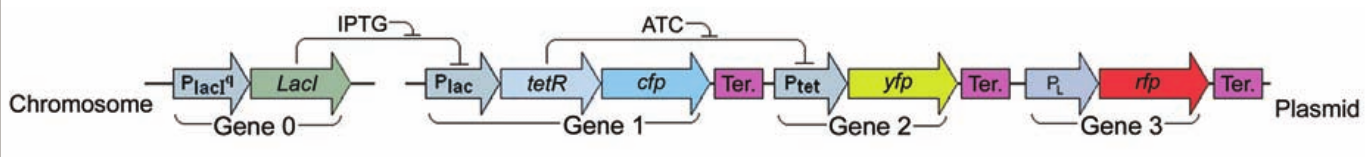
\includegraphics[width=16cm]{lan-circuit}
  \caption[Circuit used for the Langevin model]{\label{fig:lan-circuit} Circuit used in the Langevin model. From \cite{pedraza05}.}
\end{figure}

Therefore, both IPTG and ATC are environmental signals that are used to regulate the coupling between the different genes of the cascade. Notice that for instance, at higher quantities of IPTG, expression of gene $1$ is low since the repression over it is reduced. This also causes that without ATC present, the expression of gene $2$ is high. 

The fluorescent proteins are used to quantify experimentally via fluorescence microscopy the expressions of each gene, which will be proportional to the intensity of the flourescence on each color. \textit{tetR} and \textit{cfp} are transcribed bicistronically in order to be able to quantify \textit{tetR} levels. We will assume that protein degradation is caused only by cell division (i.e. there is no active degradation). That allow us to use the same degradation constant for all proteins, and in particular, to assume that the behavior of \textit{cfp} reproduces the behavior of \textit{tetR}. We will label the concentrations of \textit{LacI}, \textit{tetR} (and \textit{cfp}), \textit{yfp} and \textit{rfp} as $x_0$, $x_1$, $x_2$, and $x_3$, respectively.

\section{Mathematical derivations}

The differential equation for the mRNA will not be considered, we will write the equation for the proteins and include the effect of mRNA in the rate of creation $k$. The results of the previous chapter for the noise in proteins caused by mRNA will also be considered. The deterministic equation for the concentration of proteins of gene $0$ is 

\begin{equation}
\label{eq:detgene0}
\dot{x_0}(t) = k - \gamma x_0(t).
\end{equation}

where in this case $k$ represents the average number of proteins created per unit time\footnote{If we assume $\gamma_p\ll\gamma_r$, we can treat the mRNA in steady state, hence eq. \eqref{eq:mas-simple_det_1} becomes eq. \eqref{eq:detgene0} with $k \coloneqq k_p\langle n_1\rangle_s =  \frac{k_pk_r}{\gamma_r} = k_rb$.}.

We will use the Langevin approach following the same procedures that were explained on the previous section. Here we add two noise terms to the deterministic equations representing the intrinsic noise $\mu_0(t)$ and the global noise $\xi_0(t)$. Hence, the equation for the stochastic process $x_0(t)$ is

\begin{equation}
\label{eq:gene0}
\dot{x_0}(t) = k - \gamma x_0(t) + \mu_0(t) + \xi_0(t).
\end{equation}

The noise terms have zero average, i.e.

\begin{equation*}
\langle\mu_0\rangle(t) = \langle\xi_0\rangle(t) = 0,
\end{equation*}

and assuming white noise statistics for both sources, the autocorrelation functions are

\begin{align}
\langle\mu_0(t)\mu_0(t+\tau)\rangle&=q^2_{0,\text{int}}\delta(\tau)=2\gamma(b_0+1)\bar{x}_0\delta(\tau),\label{eq:corin0}\\
\langle\xi_0(t)\xi_0(t+\tau)\rangle&=q^2_{0,G}\delta(\tau)=2\gamma\eta_G^2\bar{x}_0^2\delta(\tau). \label{eq:corex0}
\end{align}

$\eta_G$ is the strenght of the global noise, a parameter that is measured experimentally, and $b_0$ is the average number of protein produced per mRNA. In this section the bar denotes steady state average. Also, since both sources of noise are uncorrelated

\begin{equation}
\label{eq:corinex0}
\langle\mu_0(t)\xi_0(t+\tau)\rangle = 0.
\end{equation}

We will derive the constant term in eq. \eqref{eq:corin0}. Notice that we can not use eq. \eqref{eq:lan-q_form} to find the factor $q$ in the correlations since with the assumptions made in eq. \eqref{eq:detgene0}, protein creation is not a one step Poisson process. From the results of section \ref{sec:lan-single} we obtain comparing with eq. \eqref{eq:lan-qrel1}

\begin{equation*}
  \sigma^2(x_0) = \frac{q_{0,\text{int}}^2}{2\gamma}
\end{equation*}

and from eq. \eqref{eq:lan-simple_varp} we obtain

\begin{equation*}
  \frac{q_{0,\text{int}}^2}{2\gamma}=\bar{x}_0\left(\frac{b_0}{1+\gamma_p/\gamma_r}+1\right).
\end{equation*}

The bar denotes steady state average. Since proteins are more stable than mRNA, we can approximate $\gamma_p\ll\gamma_r$ obtaining

\begin{equation*}
  q_{0,\text{int}}^2 \approx 2\gamma\bar{x}_0(b_0+1).
\end{equation*}

In fact, the factor $q_{i,\text{int}}$ has the same form for all genes, i.e.

\begin{equation*}
  q_{i,\text{int}}^2 \approx 2\gamma\bar{x}_i(b_i+1),\quad i = 0,1,2,3.
\end{equation*}

Continuing with the calculations for the noise, we will follow the same procedure as in section \ref{sec:lan-single}. In terms of $\delta x_0 \coloneqq x_0 - \bar{x}_0$, eq. \eqref{eq:gene0} becomes

\begin{equation*}
%\label{eq:dgene0}
\dot{\delta x_0}(t) = -\gamma \delta x_0(t) + \mu_0(t) + \xi_0(t).
\end{equation*}

We will Fourier transform the equation, find its square norm and use the Wiener-Khinchin theorem (eq. \eqref{eq:con-wkth}) to find the autocorrelations in terms of the power spectrum and to write the power spectrum of $\mu(t)$ and $\xi(t)$ in terms of their autocorrelations. Fourier transforming and solving for $\delta \hat{x}_0$

\begin{equation}
\label{eq:fgene0}
\delta \hat{x}_0(\omega) = \frac{\hat{\mu}_0+\hat{\xi}_0}{\gamma + i\omega}.
\end{equation}

Taking the square norm and averaging we get

\begin{equation*}
\left\langle |\delta \hat{x}_0|^2 \right\rangle = \frac{\left\langle|\hat{\mu}_0|^2\right\rangle + \left\langle\hat{\mu}_0^*\hat{\xi}_0\right\rangle+\left\langle\hat{\mu}_0\hat{\xi}_0^*\right\rangle+\left\langle|\hat{\xi}_0|^2\right\rangle}{\gamma^2 + \omega^2},
\end{equation*}

Using the Wiener-Khinchin theorem and eqs. \eqref{eq:corin0} - \eqref{eq:corinex0}

\begin{equation}
  \label{eq:pgene0}
  \begin{split}
    \left\langle |\hat{\delta x_0}|^2 \right\rangle &= \frac{\left(2\gamma(b_0+1)\bar{x_0}+ 2\gamma\eta_G^2\bar{x}_0^2\right)\mathscr{F}(\delta(t))}{\gamma^2+\omega^2}\\
    &=\frac{2\gamma\bar{x}_0^2\left(\frac{(b_0+1)}{\bar{x}_0}+ \eta_G^2\right)}{\gamma^2+\omega^2},
  \end{split}
\end{equation}

where the cross terms are zero by eq. \eqref{eq:corinex0}. Applying the inverse Fourier transform at $t=0$ we get

\begin{equation*}
\langle \delta x_0^2 \rangle = 2\gamma\bar{x}_0^2\left(\frac{(b_0+1)}{\bar{x}_0}+ \eta_G^2\right)\frac{1}{2\pi}\int_{-\infty}^{\infty}\frac{d\omega}{\omega^2+\gamma^2}
\end{equation*}

The integral can be easily solved by residues resulting in $\pi/\gamma$, then

\begin{equation*}
\langle \delta x_0^2 \rangle = \bar{x}_0^2\left(\frac{(b_0+1)}{\bar{x}_0}+ \eta_G^2\right),
\end{equation*}

and dividing by $\bar{x_0}^2$, we obtain the squared coefficient of variation

\begin{equation}
  \label{eq:etagene0}
  \eta_0^2 = \frac{(b_0+1)}{\bar{x}_0}+ \eta_G^2 = \eta_{0,\text{int}}^2+\eta_G^2,
\end{equation}

where $\eta_{i,\text{int}}^2\coloneqq\frac{(b_i+1)}{\bar{x_i}}$ for $i=0,1,2,3$. The total squared noise for gene $0$ has contributions from both the intrinsic and the global noise. Now we will find the noise for gene $1$, whose proteins follows the equation

\begin{equation}
\label{eq:gene1}
\dot{x_1} = k_1(x_{0A})-\gamma x_1+\mu_1+\xi_1
\end{equation}

The creation rate $k_1$ is a Hill equation for repression where the repressor is $x_{0A}$, the amount of $x_0$ that is unbound to IPTG. The statistics for the noise terms are analogous to eqs. \eqref{eq:corin0} - \eqref{eq:corinex0}. We also need to know in this case the correlations between the noise terms corresponding to gene $0$ and the ones corresponding to gene $1$. As we have said, extrinsic sources of noise are uncorrelated

\begin{equation}
\label{eq:corcross01}
\langle\mu_0(t)\mu_1(t+\tau)\rangle = \langle\mu_0(t)\xi_1(t+\tau)\rangle = \langle\mu_1(t)\xi_0(t+\tau)\rangle = 0,
\end{equation}

but the extrinsic parts of the noise of genes $0$ and $1$ are correlated. In analogy with eq. \eqref{eq:corex0} we get

\begin{equation*}
  \langle\xi_0(t)\xi_1(t+\tau)\rangle = 2\gamma\eta_G^2\bar{x}_0\bar{x}_1\delta(\tau).
\end{equation*}

We proceed in a similar way to gene $0$. Defining $\delta x_1(t) \coloneqq x_1(t) - \bar{x_1}$, writing eq. \eqref{eq:gene1} in terms of $\delta x_1$, $\delta x_{0A}$, and making a Taylor expansion of $k_1$ to first order in $x_{0A}$ about $\bar{x}_{0A}$ we obtain.

\begin{equation*}
\dot{\delta x_1} = k_1(\bar{x}_{0A}) + \left.\frac{dk_1(x_{0A})}{dx_{0A}}\right|_{\bar{x}_{0A}}\delta x_{0A} - \gamma(\delta x_1 + \bar{x}_1) + \mu_1 + \xi_1,
\end{equation*}

but from eq. \eqref{eq:gene1}, $\bar{x}_1 = k_1(\bar{x}_{0A})/\gamma$, hence

\begin{equation*}
  %\label{eq:dgene1}
  \dot{\delta{x_1}(t)}=c_1\delta x_{0A}-\gamma\delta x_1 + \mu_1 \xi_1,
\end{equation*}

where $c_1 \coloneqq \left.\frac{dk_1(x_{0A})}{dx_{0A}}\right|_{\bar{x_{0A}}}$. Fourier transforming and solving for $\delta \hat{x}_1$ we get

\begin{equation*}
  \delta \hat{x}_1=\frac{c_1\delta \hat{x}_{0A}+\hat{\mu}_1+\hat{\xi}_1}{\gamma + i\omega}.
\end{equation*}

Taking the square norm and averaging

\begin{equation}
  \label{eq:pgene1}
  \begin{split}
    \left\langle|\delta \hat{x}_1|^2\right\rangle &= \frac{1}{\omega^2+\gamma^2}\left(c_1\delta \hat{x}_{0A} + \hat{\mu}_1 + \hat{\xi}_1\right)\left(c_1\delta \hat{x}_{0A}^* + \hat{\mu}_1^* + \hat{\xi}_1^*\right)\\
    &=\frac{1}{\omega^2+\gamma^2}\left(c_1^2 \left\langle|\delta \hat{x}_{0A}|^2\right\rangle + c_1\left(\langle\delta \hat{x}_{0A}\hat{\xi}_1^*\rangle+\langle\delta \hat{x}_{0A}^*\hat{\xi}_1\rangle\right) +  \left\langle|\hat{\mu}_1|^2\right\rangle +  \left\langle|\hat{\xi}_1|^2\right\rangle\right)
  \end{split}
\end{equation}

Using the Wiener-Khinchin theorem and the equations for the correlations we get

\begin{align*}
  \left\langle|\hat{\mu}_1|^2\right\rangle &= 2\gamma(b_1+1)\bar{x}_1,\\
  \left\langle|\hat{\xi}_1|^2\right\rangle &= 2\gamma\eta_G^2\bar{x}_1^2,
\end{align*}

since the Fourier transform of the Dirac delta is $1$. Usually the binding and unbinding of inducers such as $IPTG$ occurs at timescales that are much smaller than the timescales of transcription and translation. Therefore, time averaging makes those fluctuations negligible. With this in mind, we will assume that the noise in $x_{0A}$ is the same as the noise in $x_0$. Then from eqs. \eqref{eq:fgene0} and \eqref{eq:pgene0} we get

\begin{align*}
\left\langle|\delta \hat{x}_{0A}|^2\right\rangle &= \frac{2\gamma\bar{x}_0^2\left(\frac{(b_0+1)}{\bar{x}_0}+ \eta_G^2\right)}{\gamma^2+\omega^2},\\
\langle\delta \hat{x}_{0A}\hat{\xi}_1^*\rangle &= \frac{1}{\gamma+i\omega}\left(\langle\hat{\mu}_0\hat{\xi}_1^*\rangle + \langle\hat{\xi}_0\hat{\xi}_1^*\rangle \right) = \frac{\langle\hat{\xi}_0\hat{\xi}_1^*\rangle}{\gamma+i\omega}\\
\langle\delta \hat{x}_{0A}^*\hat{\xi}_1\rangle &= \frac{1}{\gamma-i\omega}\left(\langle\hat{\mu}_0^*\hat{\xi}_1\rangle + \langle\hat{\xi}_0^*\hat{\xi}_1^*\rangle \right) = \frac{\langle\hat{\xi}_0^*\hat{\xi}_1\rangle}{\gamma-i\omega}
\end{align*}

Where the last step in the last two equations was made using the WK theorem and eq. \eqref{eq:corcross01}. Replacing the previous equations in eq. \eqref{eq:pgene1} and taking the inverse transform

\begin{equation*}
  \begin{split}
    \langle \delta x_1^2\rangle &= 2\gamma\bar{x}_0^2c_1^2\left(\frac{(b_0+1)}{\bar{x}_0}+ \eta_G^2\right)\frac{1}{2\pi}\int_{-\infty}^{\infty}\frac{d\omega}{(\omega^2+\gamma^2)^2}\\
    &+2\gamma\eta_G^2\bar{x_0}\bar{x}_1c_1\frac{1}{2\pi}\left(\int_{-\infty}^{\infty}\frac{d\omega}{(\gamma + i\omega)(\omega^2+\gamma^2)} + \int_{-\infty}^{\infty}\frac{d\omega}{(\gamma - i\omega)(\omega^2+\gamma^2)}\right)\\
    &+2\gamma\bar{x}_1^2 \left(\frac{(b_1+1)}{\bar{x}_1}+\eta_G^2\right)\frac{1}{2\pi}\int_{-\infty}^{\infty}\frac{d\omega}{\omega^2+\gamma^2}.
  \end{split}
\end{equation*} 

Solving the integrals in the complex plane and rearranging

\begin{equation*}
  \langle \delta x_1^2\rangle = \frac{c_1^2\bar{x}_0^2}{2\gamma^2}\left(\frac{(b_0+1)}{\bar{x}_0}+ \eta_G^2\right) + \frac{c_1\eta_G^2\bar{x}_0\bar{x}_1}{\gamma} + \bar{x}_1^2\left(\frac{(b_1+1)}{\bar{x}_1}+\eta_G^2\right).
\end{equation*}

Dividing by $\bar{x}_1^2$ yields

\begin{equation}
  \label{eq:lan-eta1_alm}
  \eta_1^2 = \frac{1}{2}\frac{c_1^2\bar{x_0}^2}{\gamma^2\bar{x}_1^2}\left(\frac{(b_0+1)}{\bar{x_0}}+ \eta_G^2\right) + \frac{c_1\bar{x_0}}{\gamma \bar{x}_1}\eta_G^2 + \frac{(b_1+1)}{\bar{x_1}}+\eta_G^2.
\end{equation}


From the definition of the logarithmic gain [eq. \eqref{eq:fdt-def_H}]

\begin{equation*}
  H_{10} = \frac{\partial \ln (\langle J_1^-\rangle/\langle J_1^+\rangle)}{\partial \ln \langle x_0\rangle}.
\end{equation*}

From eq. \eqref{eq:gene1}, we have $\langle J_1^+\rangle = k_1(\bar{x}_{0A})$ and $\langle J_i^-\rangle = \gamma \bar{x}_1$. Then,

\begin{equation*}
  H_{10} = \frac{\partial \ln\left(\frac{\gamma\bar{x}_1}{k1(\bar{x}_{0A})}\right)}{\partial \ln  \bar{x}_0} = -\frac{\frac{\gamma \bar{x}_1}{k_1(\bar{x}_{0A})}\partial\left(\frac{k_1(\bar{x}_{0A})}{\gamma \bar{x}_1}\right)}{\frac{\partial \bar{x}_{0A}}{\bar{x}_{0A}}} = -\frac{\bar{x}_{0A}}{k_1(\bar{x}_{0A})}\frac{\mathrm{d} k_1(\bar{x}_{0A})}{\mathrm{d} \bar{x}_{0A}} = -\frac{c_1 \bar{x}_{0A}}{\gamma\bar{x}_1}.
\end{equation*}

Since gene $2$ has the same dependence on the number of active proteins of gene $1$ (not bound to ATC), we have in general

\begin{equation}
  \label{lan-Hexp}
  H_{ij} = \frac{c_i \bar{x}_{jA}}{\gamma\bar{x}_i} = \frac{\bar{x}_{jA}}{\gamma\bar{x}_i}\frac{\mathrm{d}k_i(\bar{x}_{jA})}{\mathrm{d} \bar{x}_{jA}},\quad\text{for}\quad (i,j) = \{(1,0),(2,1)\}.
\end{equation}

Replacing this in eq. \eqref{eq:lan-eta1_alm} we obtain

\begin{equation}
  \label{eq:etagene1}
  \begin{split} 
    \eta_1^2 &= \eta_{1\text{int}}^2+\frac{1}{2}H_{10}^2\eta_{0\text{int}}^2+\eta_G^2\left(1+ \frac{1}{2}H_{10}^2-H_{10}\right), \\
    &= \eta_{1\text{int}}^2 + \frac{1}{2}H_{10}^2\eta_0^2+\eta_G^2\left(1-H_{10}\right).
  \end{split}
\end{equation}

where $\eta_{1\text{int}}^2 = \frac{(b_1+1)}{\bar{x_1}}$ and $\eta_0^2$ is given by eq. \eqref{eq:etagene0}.

The total noise in gene one is thus given by its intrinsic part, the noise from gene $0$ that is propagated to gene $1$ (including both its intrinsic and global part) and the global noise that enters directly into gene $1$. The factor of $1/2$ represents the time averaging since we assumed equal degradation rates for both proteins.

For gene $2$ we proceed similarly, with analogous statistics for the noise terms, the resulting noise is

\begin{equation}
  \label{eq:etagene2}
  \begin{split}
    \eta_2^2 &= \eta_{2\text{int}}^2 +  \frac{1}{2}H_{21}^2\eta_{1\text{int}}^2+\frac{3}{8}H_{21}^2H_{10}^2\eta_{0\text{int}}^2\\
    &+\eta_G^2\left(1 + \frac{1}{2}H_{21} + \frac{3}{8}H_{21}^2H_{10}^2 - H_{21} -\frac{3}{4}H_{21}^2H_{10} + \frac{1}{2}H_{21}H_{10}\right),\\
    &= \eta_{2\text{int}}^2 + \frac{1}{2}H_{21}^2\eta_1^2+\frac{1}{8}H_{21}^2H_{10}^2\eta_0^2+\eta_G^2\left(1-H_{21}-\frac{1}{4}H_{21}^2H_{10}+\frac{1}{2}H_{21}H_{10}\right).
  \end{split}
\end{equation}

Which contains the intrinsic noise of gene $2$, the contribution from the total noise of gene $1$, the contribution from the total noise of gene $0$ that is transmitted first to gene $1$ and then to gene $2$ and the global noise that enters directly. Notice that the time average factor for a two step propagation of intrinsic noise is less than $1/2$, verifying the conclusions of the previous section.

Since gene $3$ has also a constitutive promoter, its noise is given by

\begin{equation}
  \label{eq:etagene3}
  \eta_3^2 = \eta_{3\text{int}}^2+\eta_G^2.
\end{equation}

This gene was used to measure the strenght of the global noise $\eta_G$ since it is not connected with any other components. The correlations can be found in a very similar way. They are given by

\begin{equation}
  \label{eq:lan-correl}
  \begin{split}
    C_{12}&=-\frac{1}{2}H_{21}\eta_{1\text{int}}^2 -\frac{3}{8}H_{21}H_{10}^2\eta_{0\text{int}}^2+\eta_G^2\left(1-\frac{1}{2}H_{21}-\frac{1}{2}H_{10}-\frac{3}{8}H_{21}H_{10}^2 + \frac{3}{4}H_{21}H_{10}\right),\\
    C_{13}&=\eta_G^2\left(1-\frac{1}{2}H_{10}\right),\\
    C_{23}&=\eta_G^2\left(1-\frac{1}{2}H_{21}+\frac{1}{4}H_{21}H_{10}\right).
  \end{split}
\end{equation}

From the results it is clear that the noise is strongly dependent on the details of the network and on how is the interaction between the different components of the genetic circuit.

\section{Explicit expressions for the logarithmic gain}

The interactions between the genes of the cascade are mathematically represented writing the rates of creation as Hill type functions. They are given by

\begin{equation}
  \label{eq:lan-hill_g}
  \begin{split}
    k_1(y_{0A}) &= \alpha_1 + \frac{\beta_1}{1+(\frac{y_{0A}}{K_{d1}})^{h_1}},\\
    k_2(y_{1A}) &= \alpha_2 + \frac{\beta_2}{1+(\frac{y_{1A}}{K_{d2}})^{h_2}}.
\end{split}
  \end{equation}

The fraction of $y_0$ (\textit{LacI}) and $y_1$ (\textit{tetR}) that are unbound to ATC is also modeled as a Hill function i.e. $y_{0A} = k_0(IPTG)\cdot y_0$ and $y_{1A} = k_a(ATC)\cdot y_1$ where

\begin{equation}
  \begin{split}
    k_0(IPTG) &= \alpha_0 + \frac{\beta_0}{1+(\frac{IPTG}{K_{d0}})^{h_0}},\\
    k_2(y_{1A}) &= \alpha_a + \frac{\beta_a}{1+(\frac{ATC}{K_{da}})^{h_a}}.
\end{split}
  \end{equation}

To find the logarithmic gains $H_{21}$ and $H_{10}$, we use eq. \eqref{lan-Hexp} and eq. \eqref{eq:lan-hill_g} to obtain for $(i,j) = \{(1,0),(2,1)\}$

\begin{equation}
  \label{eq:lan-H_det}
  H_{ij} = \frac{\bar{x}_{jA}}{\gamma\bar{x}_i}\frac{\mathrm{d}}{\mathrm{d} \bar{x}_{jA}}\left( \alpha_i + \frac{\beta_i}{1+(\frac{\bar{x}_{jA}}{K_{di}})^{h_i}}\right) = \frac{h_i}{\beta_i k_i(\bar{x}_{jA})}\left(k_i(\bar{x}_{jA}) - \alpha_i\right) \left(\alpha_i+\beta_i-k_i(\bar{x}_{jA})\right).
\end{equation}

The values of the parameters that will be used in the following calculations and graphics can be found in github \footnote{The equations were solved and plotted using Wolfram Mathematica. The notebook, which also contains the values for the parameters can be found in \url{https://github.com/gutiloluis/61Monograph/blob/master/math/lan-analytic_solver.nb}. Most of the parameters were fitted experimentally by Pedraza and van Oudenaarden \cite{pedraza05}}. 

Replacing eqs. \eqref{eq:lan-hill_g} - \eqref{eq:lan-H_det} we obtain explicit expressions for the logarithmic gains that, given the values of the parameters can be replaced in the eqs. for the noises and correlations. Fig. \ref{fig:lan-Hs} shows the logarithmic gains as a function of [IPTG] when [ATC] = 0.

\begin{figure}[H]
  \centering
  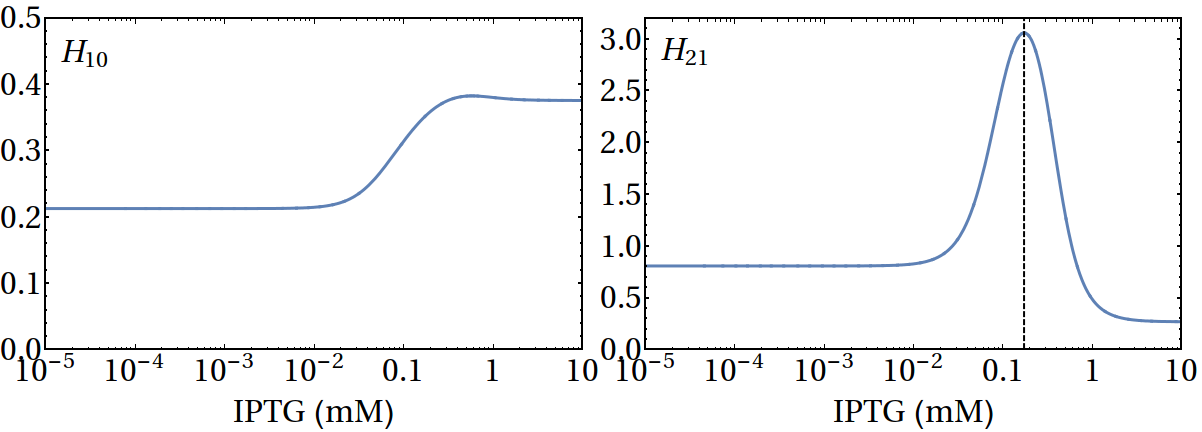
\includegraphics[width=15cm]{lan-Hs}
  \caption[Logarithmic gains for the genes of a cascade of regulation]{\label{fig:lan-Hs}. Plot of $H_{21}$ and $H_{10}$ as a function of [IPTG] given by eq. \eqref{eq:lan-H_det} . The vertical line marks the maximum of $H_{21}$.}
\end{figure}

The maximum value in $H_{21}$ represents the concentration of IPTG at which $y_2$ is more affected by changes in $y_1$. This corresponds to the point of the transfer function where the slope is greater.

Figure \ref{fig:lan-noise_corr_full} shows the noises and correlations for certain set of values of the parameters as a function of the concentration of IPTG when there is no ATC present.

\begin{figure}[H]
  \centering
  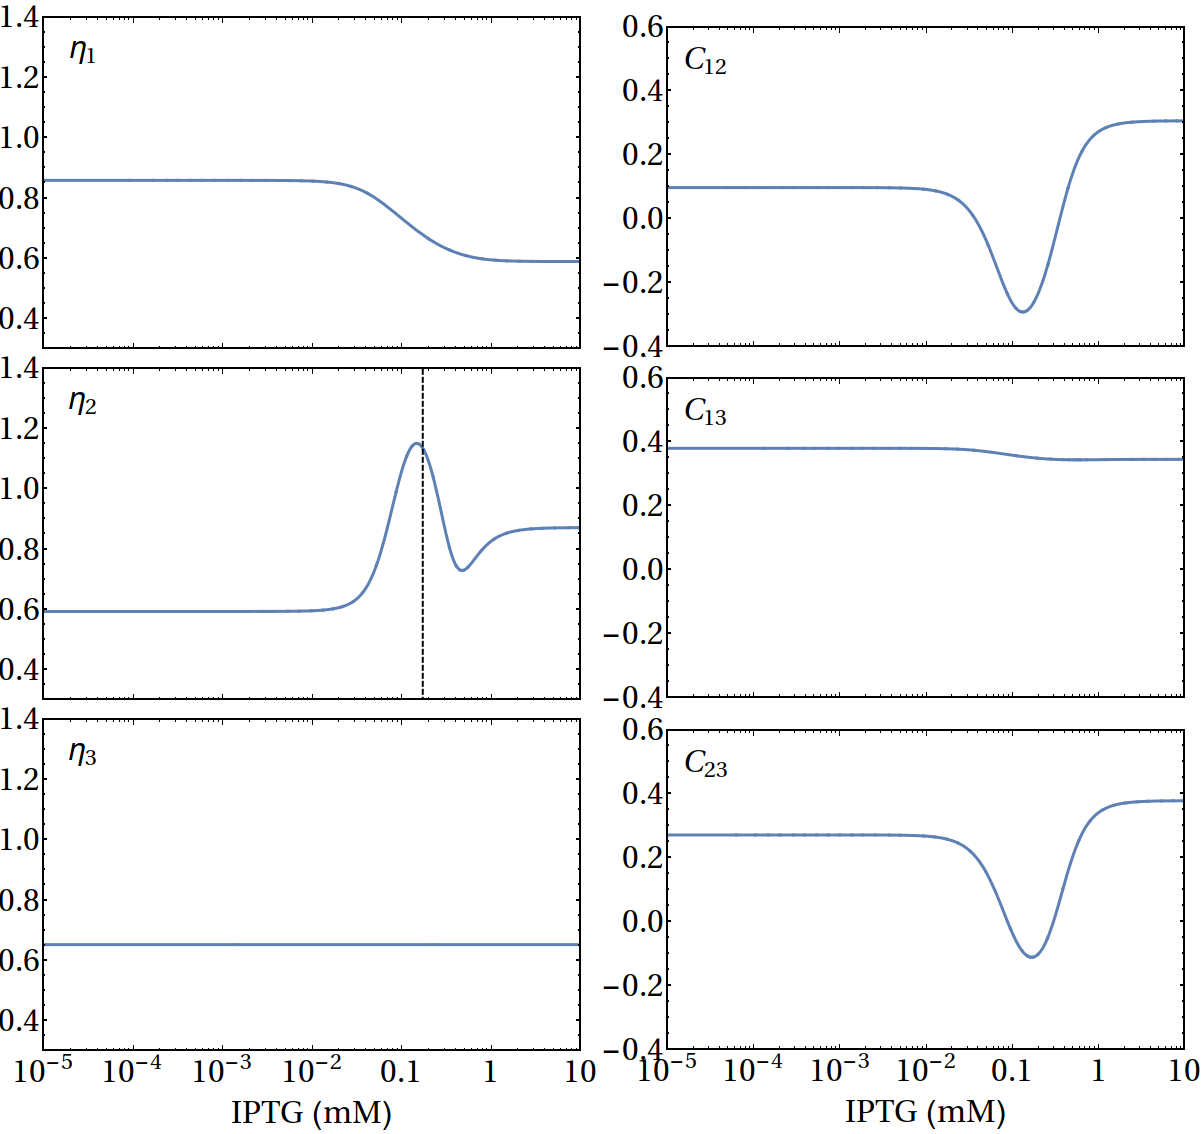
\includegraphics[width=15cm]{lan-noise_corr_full}
  \caption[Noises and correlation for the genes of a cascade of regulation]{\label{fig:lan-noise_corr_full}. Plot of noises [eqs. \eqref{eq:etagene1}-\eqref{eq:etagene3}] and correlations [eq. \eqref{eq:lan-correl}] as a function of [IPTG] for genes $1$ to $3$ with [ATC]=0. The vertical line shows the IPTG concentration at which $H_{21}$ reaches its maximum value.}
\end{figure}

The noises and correlations behave in a nonintuitive manner. For instance, $\eta_1$ and $\eta_2$ are very different altough they are both regulated by an upstream component. The correlations are also very different for each pair of genes. Recalling that gene $3$ is not regulated in the cascade, it is expected that the correlations $C_{13}$ and $C_{23}$ are independent of IPTG but the plots show that this is not the case. However, the noise for gene $3$ is constant as intuitively expected.

Another important aspect to notice is that altough there are components that do not interact directly, in the expression for the noises and correlations the interaction between them is clear. For instance, in eq. \eqref{eq:etagene2} can be seen that $\eta_2$ depends explicitely on $H_{10}$ and on the intrinsic noise of gene $0$. For this reason, noise in a regulation cascade can not be trivially added. All the upstream components contribute to the downstream components with a strenght that depends of the time average and the way the genes interact, measured by the logarithmic gain.

The vertical line in the graphic for $\eta_2$ shows that at the IPTG concentration at which $H_{21}$ is larger, the maximum of the noise almost coincides with this level. A larger value of $H$ indicates that $x_2$ is more sensitive to fluctuations in $x_1$. This explains the correspondent peak in $\eta_2$. The match is not exact due to the additional terms of eq. \eqref{eq:etagene2}. 

From eqs. \eqref{eq:etagene1} and \eqref{eq:etagene2} it can be seen that the intrinsic propagated noise always depends on the square of the logarithmic gain while the global propagated noise has terms that depend on its sign. This is a consequence of the correlation of the global noise among all the genes. For instance, a sudden change in all the creation rates caused by global noise will increase both the expressions of $x_1$ and $x_2$. Since $x_1$ represses $x_2$ this will also decrease the expression of $x_2$ proportional to the coupling between them. In the hypothetical case where $x_1$ activates $x_2$ the effect would be that the expression of $x_2$ would be increased further. In this way the correlations determine how global noise is modulated.

The previous analysis also explains the non constant correlation $C_{13}$ and $C_{23}$. Global fluctuations to gene $3$ have only the direct component, while to gene $1$ or $2$ have both the direct and transmitted component that depends on the interactions with upstream genes. Global noise will thus be reduced of increased in genes $1$ and $2$ with respect to the unregulated gene $3$ in an amount that depends on the signs and strenghts of the logarithmic gains.

Fig. \ref{fig:lan-eta2det} shows each of the components of $\eta_2$. The intrinsic squared noise varies as the inverse of the mean. When [IPTG] is large, $x_{0A}$ is small, making $x_1$ large and $x_2$ small. Therefore, the intrinsic noise should be larger as [IPTG] increases. The transmitted intrinsic noise corresponds approximately to the square of the logarithmic gain times the noise in the upstream components (including both genes $0$ and $1$). Its maximum corresponds roughly to the maximum in $H_{21}$ (vertical dashed line). The global component depends also on the correlations as explained above. When comparing the total noise with its components it becomes clear how important are the network interactions for determining the form of the noise.

\begin{figure}[H]
  \centering
  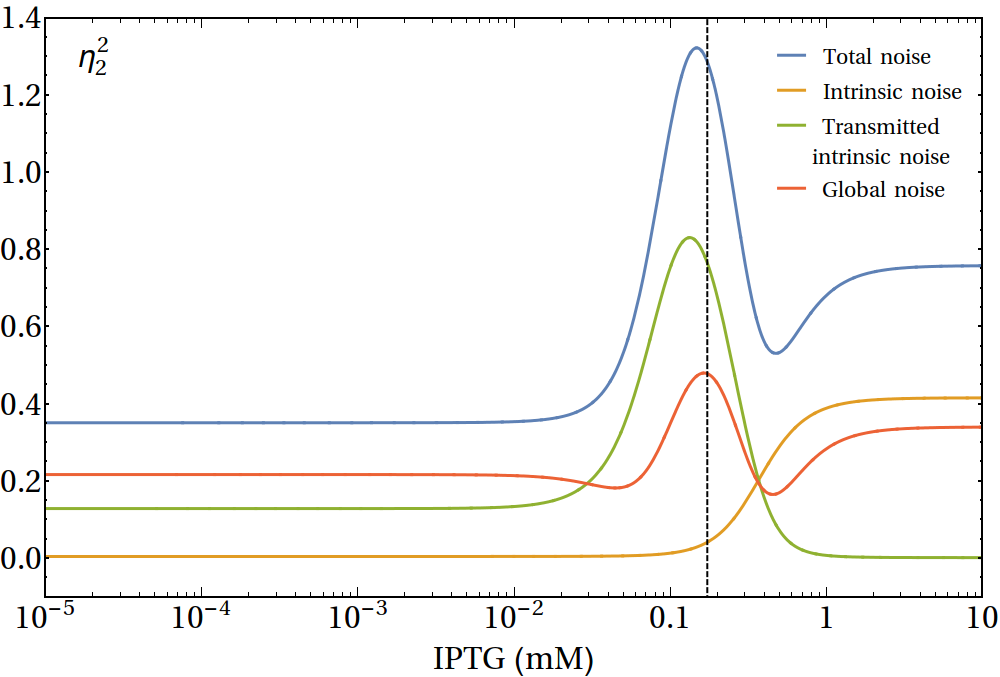
\includegraphics[width=15cm]{lan-eta2det}
  \caption[Components of the noise]{\label{fig:lan-eta2det}. Plot of each component of $\eta_2^2$ [eq. \eqref{eq:etagene2}] as a function of [IPTG] with [ATC]=0. The vertical line shows the IPTG concentration at which $H_{21}$ reaches its greater value.}
\end{figure}

The coupling between genes $1$ and $2$ is regulated with ATC. If [ATC] is large, the coupling is low and viceversa. Fig. \ref{fig:lan-eta2_corrATC} shows how $\eta_2$ and $C_{12}$ change as a function of IPTG for different [ATC] concentrations.

\begin{figure}[H]
  \centering
  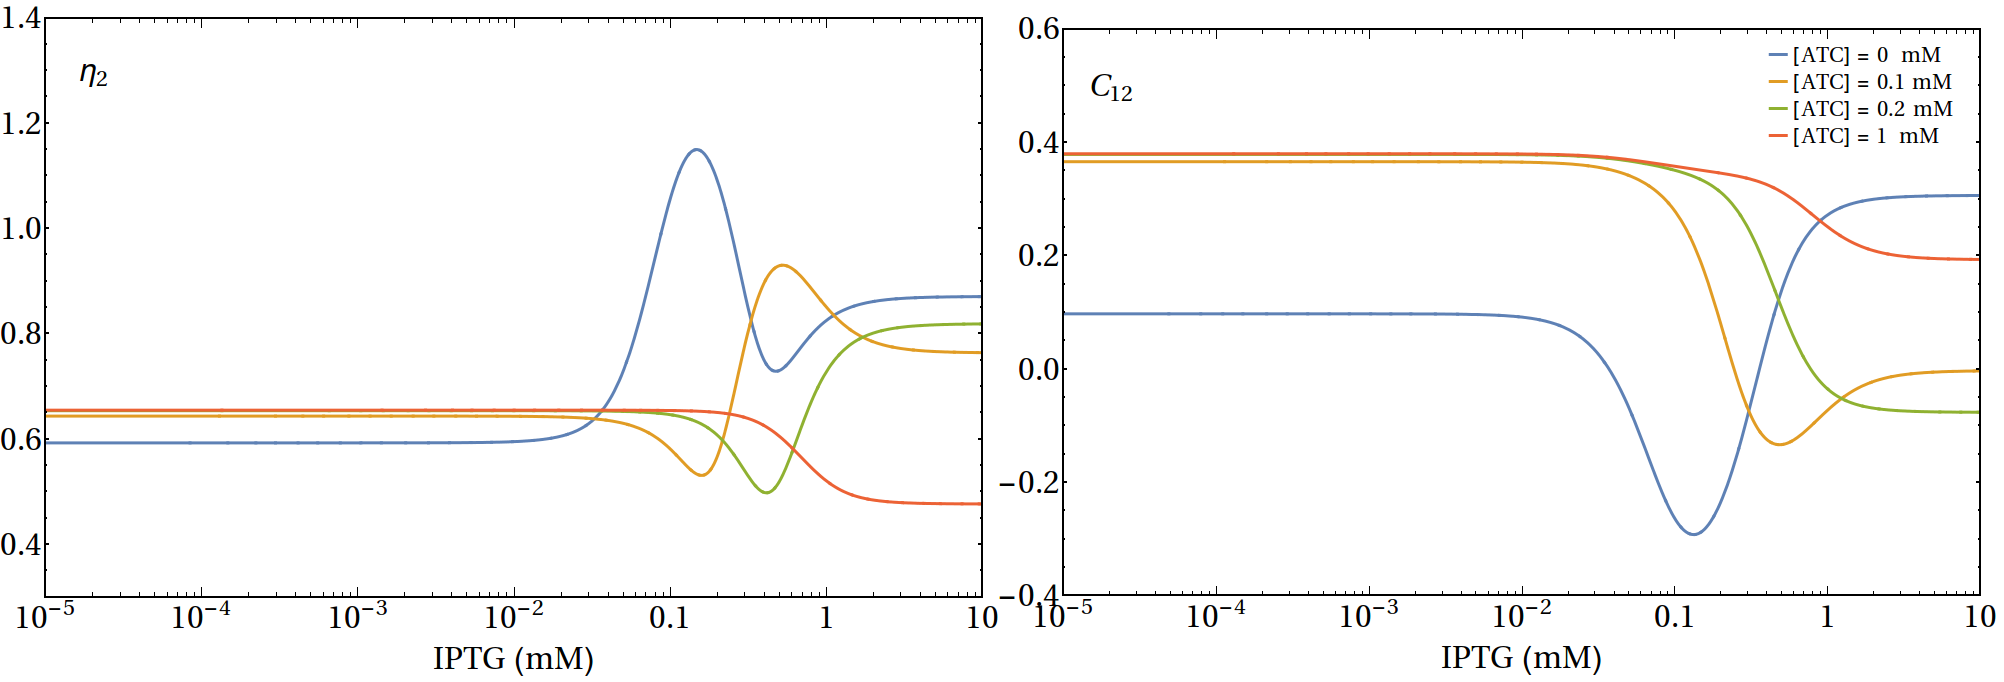
\includegraphics[width=15cm]{lan-eta2_corrATC}
  \caption[Noise in gene $2$ for varying ATC concentrations]{\label{fig:lan-eta2_corrATC}. Plots of $\eta_2$ [eq. \eqref{eq:etagene2}] and $C_{12}$ [eq. \eqref{eq:lan-correl}] as a function of [IPTG] for different ATC concentration shown in the legend.}
\end{figure}

This reconfirms the high sensitivity of the noise to the coupling of the network. For small changes in concentration of ATC, the noise shows huge changes in its behavior. At a concentration of [ATC] = $1$ mM (fig. \ref{fig:lan-eta2_corrATC}, red curve), the only considerable contributions to $\eta_2$ are the intrinsic and the directly recieved global noise.

\section{Conclusions and implications}

Fig. \ref{fig:lan-noise_sources} summarizes how noise propagates through a cascade of regulation. For the number of proteins of each gene, the noise can be decomposed on its own intrinsic noise and recieves contributions to its total noise directly from correlated global sources, and indirectly from propagated global and intrinsic fluctuations of upstream genes. The effect of the propagated noise is modulated by the logarithmic gains between the directly connected genes. Altough not shown in the figure, the time average also regulates the transmitted noise.

\begin{figure}[H]
  \centering
  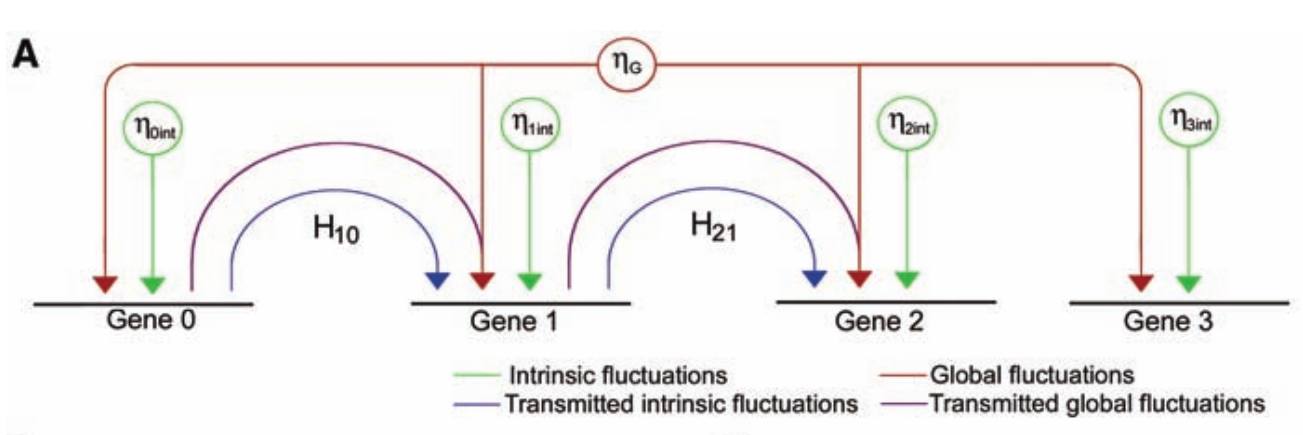
\includegraphics[width=15cm]{lan-noise_sources}
  \caption[Propagation of noise through a cascade]{\label{fig:lan-noise_sources} Different sources of noise and their propagation along the cascade of regulation (from \cite{pedraza05}).}
\end{figure}

The limitations of the model are related to the ones for the ME approach. It is also a stationary and linearized model that does not account for the time dynamics of fluctuations. In spite of that, it is remarkable how the Langevin approach enabled the authors to write the expressions for the noises in a way that is very easy to interpret. Also, the match of the experimental results with the model is excellent \cite{pedraza05} \cite{pedraza06}.

We have introduced the three basic approaches that have been used to model noise in genetic circuits: the master equation, the fluctuation-dissipation theorem and the Langevin equation. The following chapter focuses on analyzing how noise behaves when some additional factors are considered.
